\documentclass[conference]{IEEEtran}
%\IEEEoverridecommandlockouts
% The preceding line is only needed to identify funding in the first footnote. If that is unneeded, please comment it out.
\usepackage{cite}
\usepackage[caption=false,font=normalsize,labelfont=sf,textfont=sf]{subfig}
\usepackage{amsmath,amssymb,amsfonts}
\usepackage{algorithmic}
\usepackage{graphicx}
\usepackage{textcomp}
\usepackage{xcolor}
\def\BibTeX{{\rm B\kern-.05em{\sc i\kern-.025em b}\kern-.08em
    T\kern-.1667em\lower.7ex\hbox{E}\kern-.125emX}}
    \makeatletter
\newcommand{\linebreakand}{%
  \end{@IEEEauthorhalign}
  \hfill\mbox{}\par
  \mbox{}\hfill\begin{@IEEEauthorhalign}
}
\makeatother
\begin{document}

\title{Traffic Sign Classification}
%{\footnotesize \textsuperscript{*}Note: Sub-titles are not captured in Xplore and
%should not be used}
%}

%\author{\IEEEauthorblockN{Thiago de Andrade\IEEEauthorrefmark{1}, Yujuan Gao\IEEEauthorrefmark{2}, Rui Guo\IEEEauthorrefmark{3}, and Cody Haby\IEEEauthorrefmark{4}}
%\IEEEauthorblockA{\IEEEauthorrefmark{1}Department of Computer Science\\University of Florida, Gainesville, Florida 32611\\Email: tdeandradebezerr@ufl.edu}
%\IEEEauthorblockA{\IEEEauthorrefmark{2}Department of Computer Science\\University of Florida, Gainesville, Florida 32611\\Email: yujuan.gao@ufl.edu}
%\IEEEauthorblockA{\IEEEauthorrefmark{3}Department of Computer Science\\University of Florida, Gainesville, Florida 32611\\Email: rui.guo@ufl.edu}
%\IEEEauthorblockA{\IEEEauthorrefmark{4}Department of Aerospace Engineering\\University of Florida, Gainesville, Florida 32611\\Email: codyhaby@.edu}}

\author{\IEEEauthorblockN{Thiago de Andrade}
\IEEEauthorblockA{\textit{Department of Computer Science} \\
\textit{University of Florida}\\
Gainesville, Florida \\
tdeandradebezerr@ufl.edu}
\and
\IEEEauthorblockN{Yujuan Gao}
\IEEEauthorblockA{\textit{Department of Computer Science} \\
\textit{University of Florida}\\
Gainesville, Florida \\
yujuan.gao@ufl.edu}
\linebreakand
\IEEEauthorblockN{Rui Guo}
\IEEEauthorblockA{\textit{Department of Computer Science} \\
\textit{University of Florida}\\
Gainesville, Florida \\
rui.guo@ufl.edu}
\and
\IEEEauthorblockN{Cody Haby}
\IEEEauthorblockA{\textit{Department of Aerospace Engineering} \\
\textit{University of Florida}\\
Gainesville, Florida \\
codyhaby@ufl.edu}}


\maketitle

\begin{abstract}
This paper details the development of a Convolutional Neural Network (CNN), a shift invariant artificial neural network (SIANN) utilizing convolution operations instead of matrix multiplication, with the goal of classifying ten unique traffic signs. A well-balanced data set of photos with equivalent resolution was used to train and validate the neural network to determine appropriate hyperparameters for optimal performance, accurate classification greater than ninety percent. The CNN was developed using packages found within the Tensorflow library in Python, including convolution, pooling, and dense layers. Additionally, this paper documents specific experiments conducted during the design and training which led to the final architecture of the neural network. The CNN will be shown to have an accuracy of greater than ninety-four (94) percent during training and validation.
\end{abstract}

\begin{IEEEkeywords}
Machine learning, Classifier design and evaluation
\end{IEEEkeywords}

\section{Introduction}
Deep Learning algorithms have evolved in recent history to enable machines to observe their environment as humans do and utilize this knowledge to perform tasks, such as classification. A Convolutional Neural Networks (CNN) is a deep learning algorithm that can train large datasets with millions of parameters, in the form of 2D images as input, and convolve it with filters to produce the desired output\cite{b1}. CNNs are composed of convolutional layers, pooling layers, and dense layers. Convolution layers capture the spatial and temporal aspects of the input to extract high level features, with each additional/deeper layer allowing further adaptation to the high level features of the input. Pooling layers are used to reduce the spatial size of the convolved features, thus reducing the required computational power, while also extracting dominant features. Rather than requiring the user to declare the features of interest, convolutional and pooling layers work together to define, optimize, and learn the features/kernels of the input data automatically. Dense, or "Fully Connected", layers are then utilized to learn non-linear combinations of the features representing the output classification over a series of epochs with backpropagation\cite{b2}.

The architectural design of this CNN was developed through experimental design performed prior to final training. Specific experiments conducted include preprocessing strategies, training data augmentation, architecture definition, and hyperparameter tuning. Further details are available in Section \ref{sec:experiments}.

\section{Implementation}\label{sec:implementation}
The machine learning system developed follows a basic CNN architecture. The final training model used alternating convolutional layers and  pooling layers, five (5) and four (4) respectively, followed by two (2) dense layers. The convolutional layers utilized a Rectified Linear Unit (ReLU) activation function with a kernel size of thirty-two (32) for the first layer, sixty-four (64) for the following 2 layers, and one-hundred and twenty-eight (128) for the final two layers. Every pooling layers utilized "same" padding. The first dense layer used a ReLU activation with an output dimensionality of sixty-four (64) while the final dense layer, the output, used a softmax activation function with an output dimensionality of ten (10). Additionally, during training dropout regularization was used after the first set of convolutional and pooling layers with a dropout rate set to twenty percent (0.20). Adaptive Moment Optimization (Adam) was used as the optimizer in leu of gradient descent since it makes use of both momentum optimization and adaptive learning rate. Sparse categorical crossentropy was the loss function used during backpropagation to minimize the error between the actual and predicted results. The final model training used thirty (30) epochs and a batch size of thirty-two (32) to extract the high level features. The initial values of the hyperparameters for the neural network (number of hidden layers, number of neurons per layer, and the learning rate) were chosen based on literature recommendations and were then fine tuned for better performance. Unfortunately, due to issues with the University of Florida's (UF) High Performance Computing (HPC) cluster, all training/testing had to be completed locally. For this reason, typical cross-validation techniques such as GridSearchCV() and RandomizedSearchCV() could not be performed due to limited computer RAM. No attempt was made to flag signs that were not part of the baseline ten (10) classes.

To implement the model on a test set, the trained model should be loaded and the test data passed into the model. Note, the test data should be augmented equivalently to that performed on the training set.

\section{Experiments}\label{sec:experiments}

\subsection{Data Preprocessing}
\begin{figure}[htbp]
\centerline{\includegraphics{ClassPicsSmall.png}}
\caption{Class 0-9: Stop, Yield, Red Light, Green Light, Roundabout, Right Turn Only, Do Not Enter, Crosswalk, Handicap Parking, No Parking}
\label{fig_classes}
\end{figure}

Several experimental designs were performed to help define and optimize the machine learning system. These experiments were performed on both the training data and on the model to increase accuracy and decreasing computational time.

Data preprocessing was performed on the initial training set of six-thousand one-hundred and ninety-five (6,195) samples which represented the ten (10) traffic sign classes shown in Fig.~\ref{fig_classes}. Images that were mislabeled were corrected to represent the correct class. Images that did not correspond to any class and images that contained more than one class were removed from the training data.

\subsection{Data Augmentation}
\begin{figure}[htbp]
\centerline{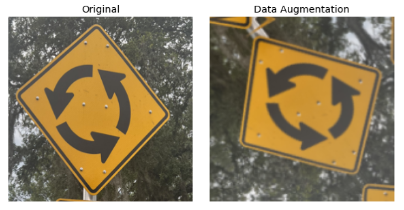
\includegraphics{DataAugmentation_Small.png}}
\caption{Original Image (Left), Augmented Image (Right)}
\label{fig_dataaug}
\end{figure}

The sequential class inside of the Keras application programming interface (API) was utilized to create linear layers to resize, rescale, randomly flip, randomly rotate, and randomly zoom in the order defined. The images new resized shape, 150x150, was an additional hyperparameter that was tuned during training. The red green blue (RGB) images were rescaled by two-hundred and fifty-five (255) so that all pixels are between zero (0) and one (1). The random flips were performed in both the vertical and horizontal planes. Random rotations equating to twenty (20) percent of one full rotation were performed in both the clockwise and counter-clockwise directions. Finally, both vertical and horizontal zooming, in and out, of twenty (20) percent were randomly performed on the images. Fig.~\ref{fig_dataaug} shows an example of an image before and after data augmentation.

\begin{table}[htbp]
\caption{Effects of Data Augmentation}
\label{table_aug}\centering
\begin{tabular}{cccc}
\hline
$Data Augmentation$&$Training$&$Testing$\\
&(\%)&(\%)\\
\hline
With&95&94\\
Without&90&82\\
\hline
\end{tabular}
\end{table}

The data augmentation's effect on classification accuracy was quantified by comparing the results of the CNN (architecture "A" detailed further in the following sections) when trained with and without augmented data. These results are shown in Table~\ref{table_aug}. The CNN that was trained with the augmented data outperformed the CNN trained without the augmented data in both training and testing accuracy.

\subsection{Neural Network Architecture}\label{architecture}
In the development of the neural network architecture, three different designs were compared. The first, architecture "A", is the CNN described previously in Section \ref{sec:implementation} and was the eventual winner with the highest accuracy. The second, architecture "B", was similar to architecture "A" with convolutional, pooling, and dense layers present. The primary difference between these two architectures was that architecture "B" stacked convolutional layers, had an additional dense layer, and used dropout regularization between each dense layer. The third architecture made use of transfer learning by utilizing the already existing Xception pre-trained model.

\begin{table}[htbp]
\caption{Neural Network Architecture Accuracy}
\label{table_arch}\centering
\begin{tabular}{ccccc}
\hline
$Architecture$&$Training$&$Testing$\\
&(\%)&(\%)\\
\hline
A&95&94\\
B&94&92\\
XCeption&96&93\\
\hline
\end{tabular}
\end{table}

Table~\ref{table_arch} details the accuracy in training and in testing that was achieved by each of the aforementioned neural network architectures. Based on these results, architecture "A" outperformed the other two models in testing. While the pre-trained XCeption model outperformed architecture "A" in training, the lower accuracy obtained by the pre-trained XCeption model in testing indicates it may be overfitting to the training data. Architecture "B" performed the worst despite the advantages of stacked convolutional layers and additional regularization techniques.

\begin{figure}[h]
\centerline{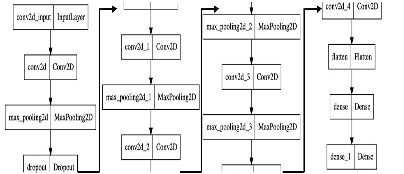
\includegraphics{Architecture_A_Small.png}}
\caption{Architecture "A"}
\label{fig_archA}
\end{figure}

Fig.~\ref{fig_archA} illustrates the final architecture selected for classification task.

\subsection{Hyperparameter Tuning}
The final experiments conducted in the design of the neural network for the classification of traffic signs was the fine tuning of hyperparameters. Hyperparameters are parameters (independent variables) whose values control the learning process and determine the values of model parameters that a learning algorithm ends up learning\cite{b3}. The hyperparameters adjusted in the design were the number of hidden layers, number of neurons per layer, and the learning rate. Additionally, the resized shape of the input pictures during data augmentation was varied.

\begin{table}[htbp]
\caption{Hyperparamater Values}
\label{table_hyp}\centering
\begin{tabular}{ccccc}
\hline
$HyperParamaters$&$Test Range$&$Final Value$\\
\hline
Image Size&UPDATE&150x150\\
Number of Hidden Layers&UPDATE&UPDATE\\
Number of Neurons per Layer&UPDATE&UPDATE\\
Learning Rate&UPDATE&0.001\\
\hline
\end{tabular}
\end{table}

Table~\ref{table_hyp} details the range of values that each hyperparamter was tested and the final value selected.

\begin{figure}[h]
\centerline{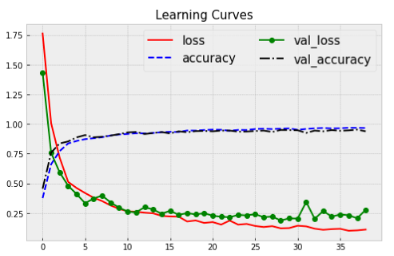
\includegraphics{LearningCurves.png}}
\caption{Learning Curves of Architecture A}
\label{fig_Learn}
\end{figure}

Fig.~\ref{fig_Learn} shows the learning curves associated with architecture "A" during training with the final hyperparameters. The accuracy increased to 95\% in training and the loss function decreased smoothly towards approximately 10\%. The loss function utilized was the sparse categorical crossentropy because due to the sparse labels (i.e., for
each instance, there is just a target class index, from 0 to 9 in this case), and the classes are exclusive.

\section{Conclusions}

\begin{thebibliography}{00}
\bibitem{b1} R. Chauhan, K. K. Ghanshala and R. C. Joshi, "Convolutional Neural Network (CNN) for Image Detection and Recognition," 2018 First International Conference on Secure Cyber Computing and Communication (ICSCCC), 2018, pp. 278-282, doi: 10.1109/ICSCCC.2018.8703316.
\bibitem{b2} S. Saha, "A Comprehensive Guide to Convolutional Neural Networks - the ELI5 way", unpublished
\bibitem{b3} K. Nyuytiymbiy, "Parameters and Hyperparameters in Machine Learning and Deep Learning", unpublished
\end{thebibliography}

%\begin{abstract}
%This document is a model and instructions for \LaTeX.
%This and the IEEEtran.cls file define the components of your paper [title, text, heads, etc.]. *CRITICAL: Do Not Use Symbols, Special Characters, Footnotes, 
%or Math in Paper Title or Abstract.
%\end{abstract}

%\section{Introduction}
%This document is a model and instructions for \LaTeX.
%Please observe the conference page limits. 

%\section{Ease of Use}

%\subsection{Maintaining the Integrity of the Specifications}

%The IEEEtran class file is used to format your paper and style the text. All margins, 
%column widths, line spaces, and text fonts are prescribed; please do not 
%alter them. You may note peculiarities. For example, the head margin
%measures proportionately more than is customary. This measurement 
%and others are deliberate, using specifications that anticipate your paper 
%as one part of the entire proceedings, and not as an independent document. 
%Please do not revise any of the current designations.

%\section{Prepare Your Paper Before Styling}
%Before you begin to format your paper, first write and save the content as a 
%separate text file. Complete all content and organizational editing before 
%formatting. Please note sections \ref{AA}--\ref{SCM} below for more information on 
%proofreading, spelling and grammar.

%Keep your text and graphic files separate until after the text has been 
%formatted and styled. Do not number text heads---{\LaTeX} will do that 
%for you.

%\subsection{Abbreviations and Acronyms}\label{AA}
%Define abbreviations and acronyms the first time they are used in the text, 
%even after they have been defined in the abstract. Abbreviations such as 
%IEEE, SI, MKS, CGS, ac, dc, and rms do not have to be defined. Do not use 
%abbreviations in the title or heads unless they are unavoidable.

%\subsection{Units}
%\begin{itemize}
%\item Use either SI (MKS) or CGS as primary units. (SI units are encouraged.) English units may be used as secondary units (in parentheses). An exception would be the use of English units as identifiers in trade, such as ``3.5-inch disk drive''.
%\item Avoid combining SI and CGS units, such as current in amperes and magnetic field in oersteds. This often leads to confusion because equations do not balance dimensionally. If you must use mixed units, clearly state the units for each quantity that you use in an equation.
%\item Do not mix complete spellings and abbreviations of units: ``Wb/m\textsuperscript{2}'' or ``webers per square meter'', not ``webers/m\textsuperscript{2}''. Spell out units when they appear in text: ``. . . a few henries'', not ``. . . a few H''.
%\item Use a zero before decimal points: ``0.25'', not ``.25''. Use ``cm\textsuperscript{3}'', not ``cc''.)
%\end{itemize}

%\subsection{Equations}
%Number equations consecutively. To make your 
%equations more compact, you may use the solidus (~/~), the exp function, or 
%appropriate exponents. Italicize Roman symbols for quantities and variables, 
%but not Greek symbols. Use a long dash rather than a hyphen for a minus 
%sign. Punctuate equations with commas or periods when they are part of a 
%sentence, as in:
%\begin{equation}
%a+b=\gamma\label{eq}
%\end{equation}

%Be sure that the 
%symbols in your equation have been defined before or immediately following 
%the equation. Use ``\eqref{eq}'', not ``Eq.~\eqref{eq}'' or ``equation \eqref{eq}'', except at 
%the beginning of a sentence: ``Equation \eqref{eq} is . . .''

%\subsection{\LaTeX-Specific Advice}

%Please use ``soft'' (e.g., \verb|\eqref{Eq}|) cross references instead
%of ``hard'' references (e.g., \verb|(1)|). That will make it possible
%to combine sections, add equations, or change the order of figures or
%citations without having to go through the file line by line.

%Please don't use the \verb|{eqnarray}| equation environment. Use
%\verb|{align}| or \verb|{IEEEeqnarray}| instead. The \verb|{eqnarray}|
%environment leaves unsightly spaces around relation symbols.

%Please note that the \verb|{subequations}| environment in {\LaTeX}
%will increment the main equation counter even when there are no
%equation numbers displayed. If you forget that, you might write an
%article in which the equation numbers skip from (17) to (20), causing
%the copy editors to wonder if you've discovered a new method of
%counting.

%{\BibTeX} does not work by magic. It doesn't get the bibliographic
%data from thin air but from .bib files. If you use {\BibTeX} to produce a
%bibliography you must send the .bib files. 

%{\LaTeX} can't read your mind. If you assign the same label to a
%subsubsection and a table, you might find that Table I has been cross
%referenced as Table IV-B3. 

%{\LaTeX} does not have precognitive abilities. If you put a
%\verb|\label| command before the command that updates the counter it's
%supposed to be using, the label will pick up the last counter to be
%cross referenced instead. In particular, a \verb|\label| command
%should not go before the caption of a figure or a table.

%Do not use \verb|\nonumber| inside the \verb|{array}| environment. It
%will not stop equation numbers inside \verb|{array}| (there won't be
%any anyway) and it might stop a wanted equation number in the
%surrounding equation.

%\subsection{Some Common Mistakes}\label{SCM}
%\begin{itemize}
%\item The word ``data'' is plural, not singular.
%\item The subscript for the permeability of vacuum $\mu_{0}$, and other common scientific constants, is zero with subscript formatting, not a lowercase letter ``o''.
%\item In American English, commas, semicolons, periods, question and exclamation marks are located within quotation marks only when a complete thought or name is cited, such as a title or full quotation. When quotation marks are used, instead of a bold or italic typeface, to highlight a word or phrase, punctuation should appear outside of the quotation marks. A parenthetical phrase or statement at the end of a sentence is punctuated outside of the closing parenthesis (like this). (A parenthetical sentence is punctuated within the parentheses.)
%\item A graph within a graph is an ``inset'', not an ``insert''. The word alternatively is preferred to the word ``alternately'' (unless you really mean something that alternates).
%\item Do not use the word ``essentially'' to mean ``approximately'' or ``effectively''.
%\item In your paper title, if the words ``that uses'' can accurately replace the word ``using'', capitalize the ``u''; if not, keep using lower-cased.
%\item Be aware of the different meanings of the homophones ``affect'' and ``effect'', ``complement'' and ``compliment'', ``discreet'' and ``discrete'', ``principal'' and ``principle''.
%\item Do not confuse ``imply'' and ``infer''.
%\item The prefix ``non'' is not a word; it should be joined to the word it modifies, usually without a hyphen.
%\item There is no period after the ``et'' in the Latin abbreviation ``et al.''.
%\item The abbreviation ``i.e.'' means ``that is'', and the abbreviation ``e.g.'' means ``for example''.
%\end{itemize}
%An excellent style manual for science writers is \cite{b7}.

%\subsection{Authors and Affiliations}
%\textbf{The class file is designed for, but not limited to, six authors.} A 
%minimum of one author is required for all conference articles. Author names 
%should be listed starting from left to right and then moving down to the 
%next line. This is the author sequence that will be used in future citations 
%and by indexing services. Names should not be listed in columns nor group by 
%affiliation. Please keep your affiliations as succinct as possible (for 
%example, do not differentiate among departments of the same organization).

%\subsection{Identify the Headings}
%Headings, or heads, are organizational devices that guide the reader through 
%your paper. There are two types: component heads and text heads.

%Component heads identify the different components of your paper and are not 
%topically subordinate to each other. Examples include Acknowledgments and 
%References and, for these, the correct style to use is ``Heading 5''. Use 
%``figure caption'' for your Figure captions, and ``table head'' for your 
%table title. Run-in heads, such as ``Abstract'', will require you to apply a 
%style (in this case, italic) in addition to the style provided by the drop 
%down menu to differentiate the head from the text.

%Text heads organize the topics on a relational, hierarchical basis. For 
%example, the paper title is the primary text head because all subsequent 
%material relates and elaborates on this one topic. If there are two or more 
%sub-topics, the next level head (uppercase Roman numerals) should be used 
%and, conversely, if there are not at least two sub-topics, then no subheads 
%should be introduced.

%\subsection{Figures and Tables}
%\paragraph{Positioning Figures and Tables} Place figures and tables at the top and 
%bottom of columns. Avoid placing them in the middle of columns. Large 
%figures and tables may span across both columns. Figure captions should be 
%below the figures; table heads should appear above the tables. Insert 
%figures and tables after they are cited in the text. Use the abbreviation 
%``Fig.~\ref{fig}'', even at the beginning of a sentence.

%\begin{table}[htbp]
%\caption{Table Type Styles}
%\begin{center}
%\begin{tabular}{|c|c|c|c|}
%\hline
%\textbf{Table}&\multicolumn{3}{|c|}{\textbf{Table Column Head}} \\
%\cline{2-4} 
%\textbf{Head} & \textbf{\textit{Table column subhead}}& \textbf{\textit{Subhead}}& \textbf{\textit{Subhead}} \\
%\hline
%copy& More table copy$^{\mathrm{a}}$& &  \\
%\hline
%\multicolumn{4}{l}{$^{\mathrm{a}}$Sample of a Table footnote.}
%\end{tabular}
%\label{tab1}
%\end{center}
%\end{table}

%\begin{figure}[htbp]
%\centerline{\includegraphics{fig1.png}}
%\caption{Example of a figure caption.}
%\label{fig}
%\end{figure}

%Figure Labels: Use 8 point Times New Roman for Figure labels. Use words 
%rather than symbols or abbreviations when writing Figure axis labels to 
%avoid confusing the reader. As an example, write the quantity 
%``Magnetization'', or ``Magnetization, M'', not just ``M''. If including 
%units in the label, present them within parentheses. Do not label axes only 
%with units. In the example, write ``Magnetization (A/m)'' or ``Magnetization 
%\{A[m(1)]\}'', not just ``A/m''. Do not label axes with a ratio of 
%quantities and units. For example, write ``Temperature (K)'', not 
%``Temperature/K''.

%\section*{Acknowledgment}

%The preferred spelling of the word ``acknowledgment'' in America is without 
%an ``e'' after the ``g''. Avoid the stilted expression ``one of us (R. B. 
%G.) thanks $\ldots$''. Instead, try ``R. B. G. thanks$\ldots$''. Put sponsor 
%acknowledgments in the unnumbered footnote on the first page.

%\section*{References}
%
%Please number citations consecutively within brackets \cite{b1}. The 
%sentence punctuation follows the bracket \cite{b2}. Refer simply to the reference 
%number, as in \cite{b3}---do not use ``Ref. \cite{b3}'' or ``reference \cite{b3}'' except at 
%the beginning of a sentence: ``Reference \cite{b3} was the first $\ldots$''
%
%Number footnotes separately in superscripts. Place the actual footnote at 
%the bottom of the column in which it was cited. Do not put footnotes in the 
%abstract or reference list. Use letters for table footnotes.
%
%Unless there are six authors or more give all authors' names; do not use 
%``et al.''. Papers that have not been published, even if they have been 
%submitted for publication, should be cited as ``unpublished'' \cite{b4}. Papers 
%that have been accepted for publication should be cited as ``in press'' \cite{b5}. 
%Capitalize only the first word in a paper title, except for proper nouns and 
%element symbols.
%
%For papers published in translation journals, please give the English 
%citation first, followed by the original foreign-language citation \cite{b6}.

%\begin{thebibliography}{00}
%\bibitem{b1} G. Eason, B. Noble, and I. N. Sneddon, ``On certain integrals of Lipschitz-Hankel type involving products of Bessel functions,'' Phil. Trans. Roy. Soc. London, vol. A247, pp. 529--551, April 1955.
%\bibitem{b2} J. Clerk Maxwell, A Treatise on Electricity and Magnetism, 3rd ed., vol. 2. Oxford: Clarendon, 1892, pp.68--73.
%\bibitem{b3} I. S. Jacobs and C. P. Bean, ``Fine particles, thin films and exchange anisotropy,'' in Magnetism, vol. III, G. T. Rado and H. Suhl, Eds. New York: Academic, 1963, pp. 271--350.
%\bibitem{b4} K. Elissa, ``Title of paper if known,'' unpublished.
%\bibitem{b5} R. Nicole, ``Title of paper with only first word capitalized,'' J. Name Stand. Abbrev., in press.
%\bibitem{b6} Y. Yorozu, M. Hirano, K. Oka, and Y. Tagawa, ``Electron spectroscopy studies on magneto-optical media and plastic substrate interface,'' IEEE Transl. J. Magn. Japan, vol. 2, pp. 740--741, August 1987 [Digests 9th Annual Conf. Magnetics Japan, p. 301, 1982].
%\bibitem{b7} M. Young, The Technical Writer's Handbook. Mill Valley, CA: University Science, 1989.
%\end{thebibliography}

\end{document}
